\documentclass{article}
\usepackage{tikz}

\begin{document}

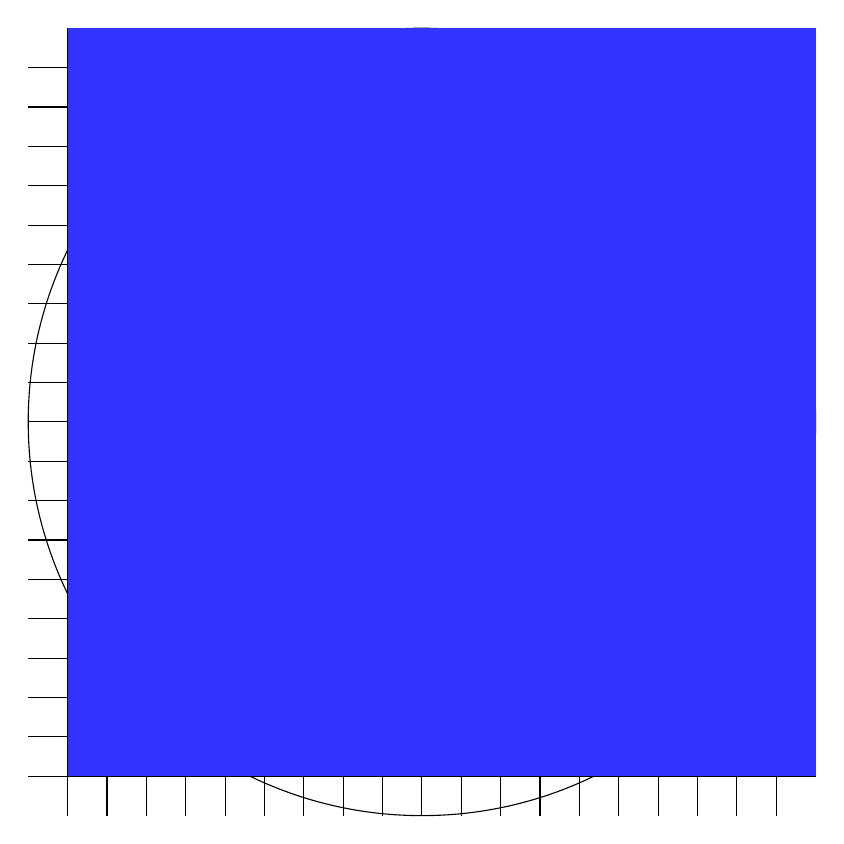
\begin{tikzpicture}[scale=0.5]
    % Draw the circle
    \draw (0,0) circle (10);
    
    % Draw the grid
    \foreach \x in {-9,...,9} {
        \draw (\x,-10) -- (\x,10);
    }
    \foreach \y in {-9,...,9} {
        \draw (-10,\y) -- (10,\y);
    }
    
    % Fill the grid with blue squares
    \foreach \x in {-9,...,9} {
        \foreach \y in {-9,...,9} {
            \fill[blue!80] (\x,\y) rectangle ++(1,1);
        }
    }
\end{tikzpicture}

\end{document}